\documentclass[tikz,border=8pt]{standalone}
\usepackage{tikz}
\usepackage{pgfplots}
\usepackage{amsmath,amssymb}
\usepackage[T1]{fontenc}
\usepackage{lmodern}
\usepackage{xcolor}
\usetikzlibrary{arrows.meta,positioning,shapes.geometric,fit,calc,backgrounds,matrix}
\pgfplotsset{compat=1.18}
\definecolor{ink}{HTML}{18202A}
\definecolor{blue}{HTML}{2563EB}
\definecolor{bluefill}{HTML}{EAF1FF}
\definecolor{green}{HTML}{14804A}
\definecolor{greenfill}{HTML}{E8F6EE}
\definecolor{amber}{HTML}{B56A00}
\definecolor{amberfill}{HTML}{FFF3D6}
\definecolor{red}{HTML}{B42318}
\definecolor{redfill}{HTML}{FDECEC}
\definecolor{gray}{HTML}{667085}
\definecolor{light}{HTML}{F4F6F8}
\definecolor{linegray}{HTML}{C7CDD4}
\tikzset{
  box/.style={draw=ink, rounded corners=3pt, very thick, fill=white, align=center, inner sep=7pt, font=\sffamily\small},
  bluebox/.style={box, fill=bluefill, draw=blue},
  greenbox/.style={box, fill=greenfill, draw=green},
  amberbox/.style={box, fill=amberfill, draw=amber},
  redbox/.style={box, fill=redfill, draw=red},
  ghost/.style={draw=linegray, rounded corners=3pt, thick, fill=light, align=center, inner sep=7pt, font=\sffamily\small},
  label/.style={font=\sffamily\footnotesize, text=gray, align=center},
  title/.style={font=\sffamily\bfseries\large, text=ink, align=center},
  arrow/.style={-{Latex[length=3mm,width=2mm]}, very thick, draw=ink},
  bluearrow/.style={-{Latex[length=3mm,width=2mm]}, very thick, draw=blue},
  redarrow/.style={-{Latex[length=3mm,width=2mm]}, very thick, draw=red},
  greenarrow/.style={-{Latex[length=3mm,width=2mm]}, very thick, draw=green}
}

\begin{document}
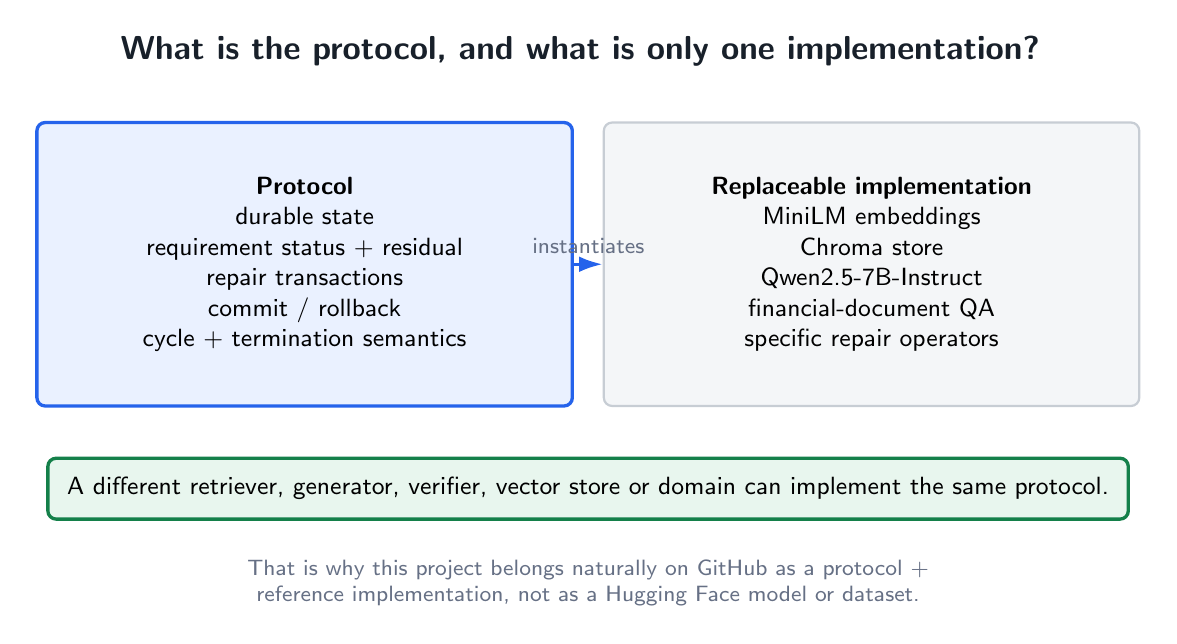
\begin{tikzpicture}
\node[title] at (7.5,5.9) {What is the protocol, and what is only one implementation?};
\node[bluebox, minimum width=68mm, minimum height=36mm] (p) at (4.0,3.2) {\textbf{Protocol}\\durable state\\requirement status + residual\\repair transactions\\commit / rollback\\cycle + termination semantics};
\node[ghost, minimum width=68mm, minimum height=36mm] (i) at (11.2,3.2) {\textbf{Replaceable implementation}\\MiniLM embeddings\\Chroma store\\Qwen2.5-7B-Instruct\\financial-document QA\\specific repair operators};
\draw[bluearrow] (p.east)--node[label,above]{instantiates}(i.west);
\node[greenbox, minimum width=130mm] at (7.6,0.35) {A different retriever, generator, verifier, vector store or domain can implement the same protocol.};
\node[label, text width=140mm] at (7.6,-0.85) {That is why this project belongs naturally on GitHub as a protocol + reference implementation, not as a Hugging Face model or dataset.};
\end{tikzpicture}
\end{document}
